% Provenance (never printed): see sources/outline_sources.md (Year 2: metamorphic reactions,
% Clapeyron slopes, the Al2SiO5 diagram, the facies grid, protoliths). Definitions and facies
% table from the IUGS subcommission proposal (via the Granada translation); thermodynamic data
% from Robie and Hemingway (1995); experimental diagram from Holdaway and Mukhopadhyay (1993);
% curves from figdata/bachelor-2/facies.py; exercise and problem values in the Book 4 scratch
% calculator calc/ch10.py.
\chapter{Reaksi dan Fasies Metamorfik}\label{ch:b2:metamorphic-facies}

Basal yang tenggelam bersama lempengnya tidak tetap menjadi basal. Plagioklas dan piroksennya
bereaksi, dalam keadaan padat, menjadi mineral lain, dan \omterm{def:b2:metamorphic-facies:assemblage}{himpunan mineral} yang baru bergantung pada
tekanan dan suhu yang dicapainya: batuan biru dari glaukofan dan lawsonit, atau
batuan hijau-merah dari omfasit dan garnet. Batuan metamorf mempertahankan mineral-mineral ini ketika
kembali ke permukaan, dan ahli petrologi yang mengenal reaksinya dapat membaca kembali
kondisi itu. Bab ini menuliskan reaksi-reaksi itu dengan termodinamika
kuliah kimia, menghitung dari data terukur diagram fase metamorfik yang paling terkenal,
yaitu diagram ketiga mineral \ce{Al2SiO5}, membandingkannya dengan percobaan, dan menata
\omterm{def:b2:metamorphic-facies:assemblage}{himpunan mineral} batuan metamorf ke dalam fasies.
% ledger: scmr:facies-assemblages

\begin{recall}
\textbf{Dari volume sekolah menengah atas}: \omterm{def:b2:metamorphic-facies:metamorphism}{metamorfisme}, derajat \omterm{def:b2:metamorphic-facies:metamorphism}{metamorfisme}, mineral indeks
dan isograd, \omterm{def:b2:metamorphic-facies:metamorphism}{metamorfisme} kontak dan aureolnya, foliasi dan skistositas,
tekanan litostatik; kianit, andalusit, dan silimanit sebagai polimorf, serta
diagram fasenya. \textbf{Dari volume Tahun 1 buku fisika dan buku kimia}: energi
Gibbs $G = H - TS$, yang minimumnya menandai keadaan stabil pada $T$ dan $P$ tertentu;
entalpi, entropi, dan kapasitas kalor; $\mathrm dG = V\,\mathrm dP - S\,\mathrm dT$;
relasi Clausius--Clapeyron untuk penguapan zat murni dan titik
tripel air. \textbf{Dari volume Tahun 1}: zona subduksi, sabuk tumbukan, dan
geoterm.
\end{recall}

\section{Metamorfisme}\label{sec:b2:metamorphic-facies:metamorphism}

Volume sekolah menengah atas mengenalkan \omterm{def:b2:metamorphic-facies:metamorphism}{metamorfisme} sebagai perubahan batuan oleh panas dan
tekanan. Sebuah rekomendasi internasional memberikan definisi yang dipakai di sini.

\begin{definition}[Metamorfisme; protolit]\label{def:b2:metamorphic-facies:metamorphism}
Yang disebut \emph{metamorfisme}\index{metamorfisme} adalah proses yang mengubah mineral atau
struktur mikro suatu batuan, atau keduanya, pada dasarnya dalam keadaan padat, ketika batuan itu menyesuaikan diri
dengan kondisi fisik yang berbeda dari kondisi saat batuan itu terbentuk dan dari kondisi yang
lazim dijumpai di permukaan Bumi dan di zona diagenesis. Proses ini dapat berlangsung bersamaan dengan
\omterm{def:b2:mantle-melting:melting}{pelelehan sebagian} dan dapat mengubah komposisi kimia batuan. Batuan sebelum
metamorfisme disebut \emph{protolit}\index{protolit}-nya.
\end{definition}
% ledger: scmr:metamorphism

Batas bawahnya mengecualikan diagenesis, yaitu perubahan sedimen ketika terkubur dan
membatu, dan batas atasnya adalah pelelehan, yang dipelajari pada \cref{ch:b2:crustal-melting}.
Agen-agennya adalah suhu, tekanan, fluida yang beredar menembus batuan (terutama air dan
karbon dioksida), dan deformasi. \omterm{def:b2:metamorphic-facies:metamorphism}{Metamorfisme} digolongkan menurut luas dan
tatanannya.
% ledger: scmr:metamorphism, scmr:types

\omterm{def:b2:metamorphic-facies:metamorphism}{Metamorfisme} \emph{regional} memengaruhi volume batuan yang besar dan menyertai proses
tektonik berskala besar: \omterm{def:b2:metamorphic-facies:metamorphism}{metamorfisme} itu bersifat \emph{orogenik} di sabuk pegunungan, tempat kerak menebal dalam
tumbukan; \omterm{def:b2:metamorphic-facies:metamorphism}{metamorfisme} \emph{penimbunan} memengaruhi batuan yang terkubur dalam di bawah tumpukan
sedimen atau vulkanik yang tebal, tanpa deformasi atau magmatisme, sehingga batuannya
biasanya tidak berskistositas; \omterm{def:b2:metamorphic-facies:metamorphism}{metamorfisme} \emph{dasar samudra} mengubah kerak di dekat
punggungan pemekaran, tempat air laut panas beredar menembusnya di bawah gradien termal
yang curam, dan rekristalisasinya biasanya tidak lengkap. \omterm{def:b2:metamorphic-facies:metamorphism}{Metamorfisme} \emph{lokal}
mempunyai penyebab setempat: \omterm{def:b2:metamorphic-facies:metamorphism}{metamorfisme} \emph{kontak} memanaskan batuan induk di sekitar suatu intrusi;
\omterm{def:b2:metamorphic-facies:metamorphism}{metamorfisme} \emph{hidrotermal} digerakkan oleh fluida panas yang kaya air;
\omterm{def:b2:metamorphic-facies:metamorphism}{metamorfisme} \emph{dislokasi}, di zona sesar dan zona geser, memperkecil ukuran butir dan
menghasilkan milonit dan kataklasit; \omterm{def:b2:metamorphic-facies:metamorphism}{metamorfisme} \emph{impak}, di bawah tumbukan \omterm{def:b2:planet-formation-meteorites:fall-find}{meteorit},
dapat melelehkan dan menguapkan batuan. \omterm{def:b2:metamorphic-facies:metamorphism}{Metamorfisme} disebut progradasi selama suhu naik dan
retrogradasi selama suhu turun.
% ledger: scmr:types

\section{Reaksi metamorfik}\label{sec:b2:metamorphic-facies:reactions}

\begin{definition}[Reaksi metamorfik; reaksi devolatilisasi]\label{def:b2:metamorphic-facies:reaction}
Yang disebut \emph{reaksi metamorfik}\index{reaksi metamorfik} adalah reaksi yang mengubah sekumpulan mineral
suatu batuan, yaitu reaktan, menjadi kumpulan lain, yaitu produk, dalam keadaan padat, mungkin
dengan keikutsertaan fase fluida. Yang disebut \emph{reaksi devolatilisasi}\index{reaksi devolatilisasi}
adalah reaksi yang melepaskan volatil, air dalam reaksi dehidrasi atau karbon
dioksida dalam reaksi dekarbonasi.
\end{definition}

Tiga jenis reaksi akan muncul dalam bab ini. Perubahan polimorf, seperti kianit menjadi
silimanit atau kalsit menjadi aragonit, mempertahankan rumus dan mengubah struktur.
Reaksi lain di antara padatan membagikan ulang komponen di antara mineral, seperti
albit yang menghasilkan jadeit dan kuarsa:
\[
\ce{NaAlSi3O8 -> NaAlSi2O6 + SiO2}.
\]
\omterm{def:b2:metamorphic-facies:reaction}{Reaksi devolatilisasi} melepaskan fluida, seperti muskovit dan kuarsa yang terurai
pada suhu tinggi:
\[
\ce{KAl3Si3O10(OH)2 + SiO2 -> KAlSi3O8 + Al2SiO5 + H2O}.
\]
% ledger: day73:ms-qz

Untuk reaksi di antara mineral yang komposisinya tetap, perubahan energi Gibbs adalah
$\Delta_r G(T, P) = \sum G_{\text{produk}} - \sum G_{\text{reaktan}}$; produk
stabil di tempat $\Delta_r G < 0$, reaktan di tempat $\Delta_r G > 0$, dan keduanya
berdampingan di tempat $\Delta_r G = 0$.

\begin{definition}[Reaksi univarian]\label{def:b2:metamorphic-facies:univariant}
Reaksi di antara fase-fase yang komposisinya tetap disebut \emph{univarian}\index{reaksi univarian}
bila syarat kesetimbangannya $\Delta_r G(T, P) = 0$ menyisakan satu variabel
bebas: kesetimbangan itu berupa garis pada bidang tekanan--suhu, yang memisahkan
medan reaktan dari medan produk.
\end{definition}

\begin{definition}[Kemiringan Clapeyron]\label{def:b2:metamorphic-facies:clapeyron}
Yang disebut \emph{kemiringan Clapeyron}\index{kemiringan Clapeyron} suatu reaksi adalah kemiringan
$\mathrm dP/\mathrm dT$ garis kesetimbangannya pada bidang tekanan--suhu.
\end{definition}

\begin{proposition}[Kemiringan Clapeyron suatu reaksi]\label{prop:b2:metamorphic-facies:clapeyron}
Di sepanjang garis kesetimbangan reaksi dengan perubahan entropi $\Delta_r S$ dan perubahan
volume $\Delta_r V$,
\[
\frac{\mathrm dP}{\mathrm dT} = \frac{\Delta_r S}{\Delta_r V}.
\]
\end{proposition}

\begin{proof}
Untuk setiap fase berlaku $\mathrm dG = V\,\mathrm dP - S\,\mathrm dT$, sehingga untuk reaksi itu
$\mathrm d(\Delta_r G) = \Delta_r V\,\mathrm dP - \Delta_r S\,\mathrm dT$. Di sepanjang garis itu
$\Delta_r G = 0$ tetap nol: $\Delta_r V\,\mathrm dP = \Delta_r S\,\mathrm dT$.
\end{proof}

Inilah relasi Clausius--Clapeyron dari fisika, yang ditulis untuk padatan. Dengan
$\Delta_r S$ dalam \unit{J.mol^{-1}.K^{-1}} dan $\Delta_r V$ dalam \unit{J.bar^{-1}} (satu
\unit{J.bar^{-1}} sama dengan \qty{10}{cm^3}), kemiringannya diperoleh dalam bar per kelvin. Dua
akibat membentuk setiap diagram fase metamorfik. Di antara padatan, perubahan entropi dan volume
kecil, sehingga garis reaksi dapat curam atau landai, positif atau
negatif: sisi suhu tinggi memuat produk yang entropinya lebih tinggi, dan
sisi tekanan tinggi memuat produk yang volumenya lebih kecil. Dalam \omterm{def:b2:metamorphic-facies:reaction}{reaksi devolatilisasi}, fluida
membawa entropi yang besar, sehingga produk terletak di sisi suhu tinggi; dan volume
fluida, yang besar pada tekanan rendah dan menyusut ketika tekanan naik, membuat kemiringannya
landai pada tekanan rendah dan lebih curam pada tekanan tinggi. Garis reaksi itu melengkung.
Percobaan pada muskovit dan kuarsa menempatkannya pada 603, 637, dan \qty{662}{\celsius} pada 1,
2, dan \qty{3}{kbar} tekanan air: antara 1 dan \qty{2}{kbar} garis itu naik
\qty{29}{bar} per kelvin, antara 2 dan 3, \qty{40}{bar} (\cref{exo:b2:metamorphic-facies:9}).
% ledger: day73:ms-qz

\section{Aluminosilikat}\label{sec:b2:metamorphic-facies:al2sio5}

\begin{definition}[Polimorf aluminosilikat]\label{def:b2:metamorphic-facies:al2sio5}
Yang disebut \emph{polimorf aluminosilikat}\index{polimorf aluminosilikat} adalah ketiga
mineral berumus \ce{Al2SiO5}: kianit (triklin), andalusit, dan silimanit (keduanya
ortorombik).
\end{definition}
% ledger: rh95:al2sio5

Mineral-mineral itu lazim dalam batu lumpur yang termetamorfosis, yang aluminiumnya dibawa oleh mineral itu, dan karena
rumusnya sama, mineral mana yang tumbuh hanya bergantung pada tekanan dan suhu. Tabel
di bawah memberikan sifat-sifat terukurnya.

\begin{center}
\small
\begin{tabular}{@{}lrrrr@{}}
\hline
 & $\Delta_f H^\circ$ (\unit{kJ.mol^{-1}}) & $S^\circ$ (\unit{J.mol^{-1}.K^{-1}}) & $V^\circ$ (\unit{J.bar^{-1}}) & massa jenis (\unit{g.cm^{-3}})\\
\hline
kianit & $-2593.8$ & 82.80 & 4.415 & 3.670\\
andalusit & $-2589.9$ & 91.39 & 5.152 & 3.145\\
silimanit & $-2586.1$ & 95.40 & 4.986 & 3.250\\
\hline
\end{tabular}
\par\smallskip{\small Kianit, andalusit, dan silimanit pada \qty{298.15}{K} dan
\qty{1}{bar} (Robie dan Hemingway, 1995); ketidakpastian entalpinya
\qty{2.0}{kJ.mol^{-1}}, ketidakpastian entropinya 0.5. Massa jenis dihitung dari massa molar,
\qty{162.046}{g.mol^{-1}}, dan volumenya.}
\end{center}
% ledger: rh95:al2sio5

Kianit paling rapat dan entropinya paling kecil: kianit adalah polimorf bertekanan tinggi dan
bersuhu rendah. Andalusit, yang paling tidak rapat, menempati tekanan rendah; silimanit,
yang entropinya paling tinggi, menempati suhu tinggi. Garis-garis kesetimbangannya dapat dihitung.

\begin{method}[Menghitung garis reaksi]\label{met:b2:metamorphic-facies:line}
(1) Dari tabel, bentuklah $\Delta_r H$, $\Delta_r S$, dan $\Delta_r V$ pada \qty{298.15}{K}
dan \qty{1}{bar}. (2) Abaikan perubahan $\Delta_r H$ dan $\Delta_r S$ terhadap
suhu (kapasitas kalor produk dan reaktan hampir sama) dan perubahan $\Delta_r V$
terhadap tekanan dan suhu (padatan hampir tidak memampat atau memuai):
\[
\Delta_r G(T, P) \approx \Delta_r H - T\,\Delta_r S + \Delta_r V\,(P - 1).
\]
(3) Samakan dengan nol: $P = 1 + (T\,\Delta_r S - \Delta_r H)/\Delta_r V$, sebuah garis lurus dengan
kemiringan $\Delta_r S/\Delta_r V$. (4) Bila ketelitian penting, gantilah $\Delta_r H$ dan
$\Delta_r S$ dengan nilainya pada suhu $T$, dari tabel $H_T - H_{298}$ dan $S_T$,
lalu selesaikan lagi. (5) Pertahankan hanya bagian setiap garis tempat kedua fasenya lebih stabil
daripada fase ketiga mana pun.
\end{method}

Untuk kianit menjadi andalusit, $\Delta_r H = \qty{3.9}{kJ}$, $\Delta_r S =
\qty{8.59}{J.K^{-1}}$, dan $\Delta_r V = \qty{0.737}{J.bar^{-1}}$: pada \qty{25}{\celsius}
dan \qty{1}{bar}, $\Delta_r G = 3900 - 298.15\times8.59 = \qty{+1.34}{kJ}$, sehingga kianit,
bukan andalusit, adalah polimorf yang stabil di permukaan Bumi; kianit menjadi silimanit memiliki
$\Delta_r G = \qty{+3.94}{kJ}$ di sana. Kemiringannya adalah $8.59/0.737 = \qty{11.7}{bar/K}$ untuk
kianit menjadi andalusit, $12.60/0.571 = \qty{22.1}{bar/K}$ untuk kianit menjadi silimanit, dan
$4.01/(-0.166) = \qty{-24.2}{bar/K}$ untuk andalusit menjadi silimanit, satu-satunya reaksi dari
ketiganya yang produk suhu tingginya lebih rapat.
% ledger: rh95:al2sio5

\begin{definition}[Titik invarian]\label{def:b2:metamorphic-facies:invariant}
Yang disebut \emph{titik invarian}\index{titik invarian} adalah titik pada bidang
tekanan--suhu tempat tiga fase atau lebih dari suatu sistem berdampingan dalam
kesetimbangan dan semua garis \omterm{def:b2:metamorphic-facies:univariant}{univarian} di antaranya bertemu; tidak ada variabel yang bebas di sana.
\end{definition}

\begin{proposition}[Titik tripel]\label{prop:b2:metamorphic-facies:triple}
Ketiga garis kianit $=$ andalusit, kianit $=$ silimanit, dan andalusit $=$
silimanit bertemu di satu titik. Di sekitarnya, setiap garis hanya stabil pada satu sisi; perpanjangan
metastabilnya terletak di medan polimorf ketiga.
\end{proposition}

\begin{proof}
Untuk setiap $(T, P)$, $\Delta G_{\text{ky}\to\text{sil}} = \Delta G_{\text{ky}\to\text{and}} +
\Delta G_{\text{and}\to\text{sil}}$, karena energi Gibbs andalusit saling meniadakan. Di tempat
dua garis pertama berpotongan, dua dari suku-suku ini bernilai nol, sehingga suku ketiga juga: garis ketiga
melalui titik potong itu. Di seberang titik potong, misalnya pada garis kianit $=$ andalusit,
$G_{\text{ky}} = G_{\text{and}}$, tetapi titik itu terletak di sisi silimanit dari
dua garis lainnya, sehingga $G_{\text{sil}}$ lebih kecil daripada keduanya: baik kianit maupun andalusit
tidak stabil di sana, dan garis itu metastabil.
\end{proof}

Dengan sifat-sifat konstan menurut metode tadi, titik tripel terletak pada
\qty{514}{\celsius} dan \qty{3.88}{kbar} (soal akhir pekan); dengan ketergantungan pada suhu
menurut tabel, pada \qty{536}{\celsius} dan \qty{4.20}{kbar}. Diagram
eksperimental, yang dibangun dari percobaan bolak-balik, menempatkannya pada $504 \pm \qty{20}{\celsius}$ dan
$3.75 \pm \qty{0.25}{kbar}$ (gambar di bawah).
% ledger: rh95:al2sio5-ht, hm93:triple, hm93:table11

\begin{omfigure}
\centering
\begin{tikzpicture}
\begin{axis}[omrecord, width=0.84\linewidth, height=7.4cm,
  xmin=200, xmax=900, ymin=0, ymax=10, xlabel={$T$ (\unit{\celsius})}, ylabel={$P$ (\unit{kbar})},
  legend style={font=\scriptsize, at={(0.02,0.98)}, anchor=north west},
  tick label style={font=\scriptsize}, label style={font=\small}]
\addplot[very thick, blue!70!black] table[x=T_C, y=P_kbar] {figdata/out/bachelor-2-facies-stable-kyand.dat};
\addlegendentry{terhitung (tabel)}
\addplot[thick, gray, densely dashed, mark=o, mark size=1.2pt] table[x=T_C, y=P_kbar] {figdata/out/bachelor-2-facies-hm93-kyand.dat};
\addlegendentry{eksperimental}
\addplot[thick, orange!85!black, mark=square*, mark size=1.3pt] table[x=T_C, y=P_kbar] {figdata/out/bachelor-2-facies-day73.dat};
\addlegendentry{muskovit + kuarsa}
\addplot[very thick, blue!70!black, forget plot] table[x=T_C, y=P_kbar] {figdata/out/bachelor-2-facies-stable-kysil.dat};
\addplot[very thick, blue!70!black, forget plot] table[x=T_C, y=P_kbar] {figdata/out/bachelor-2-facies-stable-andsil.dat};
\addplot[thin, blue!70!black, dashed, forget plot] table[x=T_C, y=P_kbar] {figdata/out/bachelor-2-facies-meta-kyand.dat};
\addplot[thin, blue!70!black, dashed, forget plot] table[x=T_C, y=P_kbar] {figdata/out/bachelor-2-facies-meta-kysil.dat};
\addplot[thin, blue!70!black, dashed, forget plot] table[x=T_C, y=P_kbar] {figdata/out/bachelor-2-facies-meta-andsil.dat};
\addplot[thick, gray, densely dashed, mark=o, mark size=1.2pt, forget plot] table[x=T_C, y=P_kbar] {figdata/out/bachelor-2-facies-hm93-kysil.dat};
\addplot[thick, gray, densely dashed, mark=o, mark size=1.2pt, forget plot] table[x=T_C, y=P_kbar] {figdata/out/bachelor-2-facies-hm93-andsil.dat};
\addplot[only marks, mark=*, mark size=2pt, blue!70!black, forget plot] table[x=T_C, y=P_kbar] {figdata/out/bachelor-2-facies-triple-B.dat};
\addplot[only marks, mark=*, mark size=2pt, gray, forget plot] table[x=T_C, y=P_kbar] {figdata/out/bachelor-2-facies-hm93-triple.dat};
\node[font=\small\bfseries] at (axis cs:330,6.2) {kianit};
\node[font=\small\bfseries] at (axis cs:460,0.6) {andalusit};
\node[font=\small\bfseries] at (axis cs:790,3.6) {silimanit};
\end{axis}
\end{tikzpicture}
\par\smallskip{\small Diagram \ce{Al2SiO5} yang dihitung dari tabel termodinamika
Robie dan Hemingway (1995) dengan entalpi dan entropi yang bergantung pada suhu (biru; putus-putus:
perpanjangan metastabil), dan diagram eksperimental Holdaway dan Mukhopadhyay (1993)
(kelabu, titik-titik tabulasinya). Jingga: penguraian muskovit + kuarsa yang diukur oleh
Day (1973), yang melengkung.}
\end{omfigure}
% ledger: rh95:al2sio5, rh95:al2sio5-ht, hm93:table11, hm93:triple, day73:ms-qz

Garis kianit--andalusit yang terhitung jatuh dalam selisih \qty{0.1}{kbar} dari garis eksperimental
antara 400 dan \qty{600}{\celsius}, tetapi garis andalusit--silimanit terletak
\qty{0.65}{kbar} terlalu tinggi pada \qty{600}{\celsius}. Garis itu yang paling rapuh di antara
ketiganya: dengan $\Delta_r V = \qty{-0.166}{J.bar^{-1}}$, galat \qty{0.1}{kJ} pada
$\Delta_r H$, yaitu seperdua puluh ketidakpastian setiap entalpi dalam tabel, menggesernya sejauh
\qty{600}{bar}. Entalpi dalam tabel itu sendiri disesuaikan agar cocok dengan
percobaan, dalam batas ketidakpastiannya; percobaanlah, bukan kalorimetri saja, yang menetapkan
diagram itu.
% ledger: rh95:al2sio5, hm93:adjusted, hm93:table11

Gambar di bawah memperlihatkan mengapa sebuah garis menjadi batas. Pada \qty{6}{kbar}, energi Gibbs
andalusit dan silimanit, yang diukur dari energi Gibbs kianit, melintasi nol di tempat masing-masing
menjadi lebih stabil daripada kianit; selisihnya tidak pernah melebihi beberapa kilojoule per mol,
itulah sebabnya galat kecil pada entalpi menggeser garis sejauh itu.

\begin{omfigure}
\centering
\begin{tikzpicture}
\begin{axis}[omrecord, width=0.7\linewidth, height=5.4cm,
  xmin=300, xmax=900, ymin=-4, ymax=4.5, xlabel={$T$ (\unit{\celsius})},
  ylabel={$G - G_{\text{kianit}}$ (\unit{kJ.mol^{-1}})},
  legend style={font=\scriptsize, at={(0.02,0.02)}, anchor=south west},
  tick label style={font=\scriptsize}, label style={font=\small}]
\addplot[very thick, red!75!black] table[x=T_C, y=dG_and] {figdata/out/bachelor-2-facies-dg6.dat};
\addlegendentry{andalusit}
\addplot[very thick, green!45!black] table[x=T_C, y=dG_sil] {figdata/out/bachelor-2-facies-dg6.dat};
\addlegendentry{silimanit}
\addplot[thin, black] coordinates {(300,0) (900,0)};
\end{axis}
\end{tikzpicture}
\par\smallskip{\small Energi Gibbs andalusit dan silimanit relatif terhadap kianit pada
\qty{6}{kbar}, dari tabel yang sama. Kianit stabil selama kedua kurva positif;
silimanit mengambil alih pada \qty{624}{\celsius}. Andalusit baru melintasi nol pada
\qty{692}{\celsius}, ketika silimanit sudah lebih rendah: di atas tekanan
titik tripel, andalusit tidak pernah menjadi yang paling stabil.}
\end{omfigure}
% ledger: rh95:al2sio5, rh95:al2sio5-ht

\begin{inthelab}[Membalik reaksi]
Garis reaksi ditentukan letaknya di laboratorium melalui percobaan pada tekanan dan
suhu tetap yang dimulai dari campuran reaktan dan produk. Dalam alat piston--silinder,
campuran itu ditahan selama satu sampai beberapa hari; arah reaksi lalu
dibaca dari difraksi sinar-X, dengan membandingkan rasio puncak produk dan reaktan
dengan rasio pada campuran awal, dan ditegaskan oleh pertumbuhan lapisan baru pada mineral yang stabil. Penelitian
lain menimbang satu kristal andalusit yang direaksikan dalam serbuk kianit atau
silimanit, dengan mikroneraca yang teliti sampai sekitar \qty{4}{\micro g}. Suatu kesetimbangan
disebut \emph{terbalikkan} bila pertumbuhan masing-masing sisi telah teramati di kedua sisi garis;
garis itu lalu terletak di dalam rentang di antaranya, yang digambar dengan galat alatnya,
biasanya \qty{10}{\celsius} dan \qty{0.5}{kbar}. Para peneliti eksperimental menilai diagram fase pertama-tama
dari pembalikan semacam itu, dan baru kemudian dari batuannya.
\end{inthelab}
% ledger: hm93:methods

\section{Himpunan mineral dan fasies}\label{sec:b2:metamorphic-facies:facies}

\begin{definition}[Himpunan mineral]\label{def:b2:metamorphic-facies:assemblage}
Yang disebut \emph{himpunan mineral}\index{himpunan mineral} adalah kumpulan mineral yang tumbuh
bersama dalam kesetimbangan di dalam batuan metamorf.
\end{definition}

\omterm{def:b2:metamorphic-facies:assemblage}{Himpunan mineral} bergantung pada kondisi \omterm{def:b2:metamorphic-facies:metamorphism}{metamorfisme} dan pada komposisi
batuan. Eskola, yang memperkenalkan konsep fasies pada 1915, melihat bahwa batuan yang
komposisinya sama membawa \omterm{def:b2:metamorphic-facies:assemblage}{himpunan mineral} yang sama pada kondisi yang sama, dan bahwa
\omterm{def:b2:metamorphic-facies:assemblage}{himpunan mineral} batuan yang berbeda berubah bersama ketika kondisinya berubah;
rekomendasi internasional mempertahankan konsepnya.
% ledger: scmr:facies

\begin{definition}[Fasies metamorfik; kisi fasies]\label{def:b2:metamorphic-facies:facies}
Yang disebut \emph{fasies metamorfik}\index{fasies metamorfik} adalah sekumpulan \omterm{def:b2:metamorphic-facies:assemblage}{himpunan mineral}
metamorfik yang berulang kali berasosiasi dalam ruang dan waktu, yang menunjukkan hubungan teratur
antara komposisi mineral dan komposisi kimia total, sehingga fasies yang berbeda
bersesuaian dengan kondisi \omterm{def:b2:metamorphic-facies:metamorphism}{metamorfisme} yang berbeda, terutama suhu dan tekanan.
Fasies dinamai dan didefinisikan berdasarkan \omterm{def:b2:metamorphic-facies:assemblage}{himpunan mineral} batuan yang berkomposisi basaltik. Yang disebut
\emph{kisi fasies}\index{kisi fasies} adalah susunan fasies pada
bidang tekanan--suhu.
\end{definition}
% ledger: scmr:facies

Tabel di bawah mendaftar sepuluh fasies berdasarkan mineral diagnostiknya dalam metabasal.

\begin{center}
\small
\begin{tabular}{@{}p{0.27\linewidth}p{0.66\linewidth}@{}}
\hline
fasies & mineral diagnostik metabasal\\
\hline
zeolit & zeolit seperti laumontit dan heulandit\\
prehnit--pumpelliit & prehnit + pumpelliit, prehnit + aktinolit, pumpelliit + aktinolit\\
sekis hijau & aktinolit + albit + klorit + epidot\\
amfibolit epidot & hornblende + albit + epidot $\pm$ klorit\\
amfibolit & hornblende + plagioklas (anortit lebih dari \qty{17}{\percent})\\
granulit & klinopiroksen + ortopiroksen + plagioklas; olivin tidak stabil bersama plagioklas atau garnet\\
sekis biru & glaukofan + epidot $\pm$ garnet, atau glaukofan + lawsonit\\
eklogit & omfasit + garnet; plagioklas tidak stabil\\
\omterm{def:b2:magma-emplacement:aureole}{hornfels} piroksen & klinopiroksen + ortopiroksen + plagioklas; olivin stabil bersama plagioklas\\
sanidinit & sama seperti di atas, dengan mineral bersuhu sangat tinggi seperti pigeonit\\
\hline
\end{tabular}
\par\smallskip{\small Fasies dan \omterm{def:b2:metamorphic-facies:assemblage}{himpunan mineral} diagnostiknya dalam batuan berkomposisi
basaltik, menurut rekomendasi internasional (delapan fasies Eskola, dengan
fasies zeolit dan fasies prehnit--pumpelliit yang ditambahkan kemudian).}
\end{center}
% ledger: scmr:facies-assemblages, scmr:facies

Rekomendasi itu menekankan apa yang tidak dilakukan fasies: fasies merekam keteraturan di antara
\omterm{def:b2:metamorphic-facies:assemblage}{himpunan mineral}, dan tidak berusaha menetapkan tekanan dan suhu masing-masing. Urutannya pada
bidang tekanan--suhu mengikuti reaksi-reaksi di antara fasies itu, dan
gambar di bawah menggambarkannya secara skematis. Suhu meningkat dari fasies zeolit melalui
fasies sekis hijau dan amfibolit sampai fasies granulit; pada tekanan rendah dan suhu
tinggi terletak fasies \omterm{def:b2:magma-emplacement:aureole}{hornfels} di \omterm{def:b2:magma-emplacement:aureole}{aureol kontak}; pada tekanan tinggi dan suhu
rendah, fasies sekis biru; pada tekanan tinggi dan suhu yang lebih tinggi, fasies
eklogit. Reaksi-reaksi dalam bab ini menetapkan sebagian batas-batas itu: plagioklas, yang
hadir sebagai albit atau sebagai plagioklas yang lebih kalsik dari fasies sekis hijau sampai fasies granulit,
tidak stabil dalam fasies eklogit, seperti yang ditunjukkan
albitnya ketika berubah menjadi jadeit dan kuarsa (\cref{exo:b2:metamorphic-facies:8}); kalsit berubah menjadi
aragonit yang lebih rapat pada tekanan tinggi (\cref{exo:b2:metamorphic-facies:7}).
% ledger: scmr:facies, scmr:facies-assemblages

\begin{omfigure}
\centering
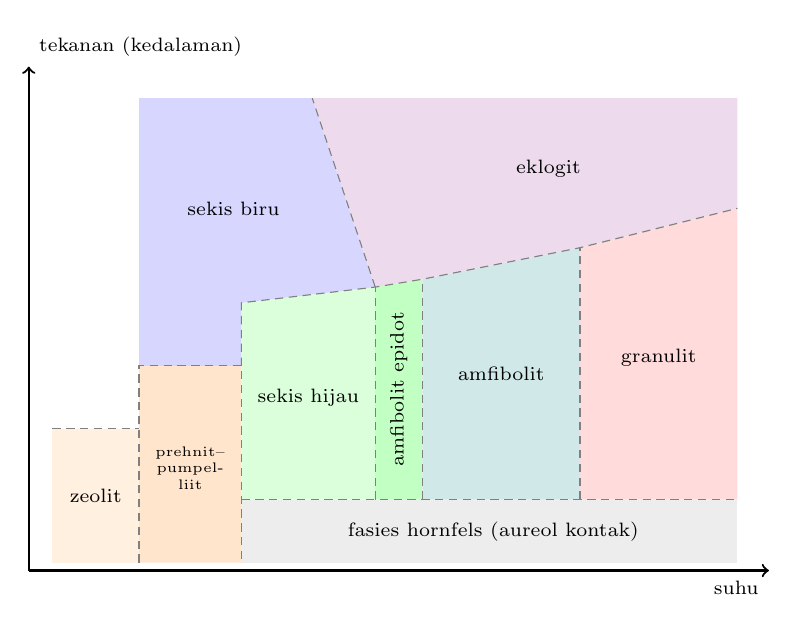
\begin{tikzpicture}[font=\scriptsize, x=1cm, y=1cm]
\draw[->, thick] (0,0) -- (9.4,0) node[below left] {suhu};
\draw[->, thick] (0,0) -- (0,6.4) node[above right] {tekanan (kedalaman)};
\fill[orange!12] (0.3,0.1) -- (1.4,0.1) -- (1.4,1.8) -- (0.3,1.8) -- cycle;
\fill[orange!20] (1.4,0.1) -- (2.7,0.1) -- (2.7,2.6) -- (1.4,2.6) -- (1.4,1.8) -- cycle;
\fill[green!14] (2.7,0.9) -- (4.4,0.9) -- (4.4,3.6) -- (2.7,3.4) -- cycle;
\fill[green!24] (4.4,0.9) -- (5.0,0.9) -- (5.0,3.7) -- (4.4,3.6) -- cycle;
\fill[teal!18] (5.0,0.9) -- (7.0,0.9) -- (7.0,4.1) -- (5.0,3.7) -- cycle;
\fill[red!14] (7.0,0.9) -- (9.0,0.9) -- (9.0,4.6) -- (7.0,4.1) -- cycle;
\fill[gray!14] (2.7,0.1) -- (9.0,0.1) -- (9.0,0.9) -- (2.7,0.9) -- cycle;
\fill[blue!16] (1.4,2.6) -- (2.7,2.6) -- (2.7,3.4) -- (4.4,3.6) -- (3.6,6.0) -- (1.4,6.0) -- cycle;
\fill[violet!14] (4.4,3.6) -- (5.0,3.7) -- (7.0,4.1) -- (9.0,4.6) -- (9.0,6.0) -- (3.6,6.0) -- cycle;
\draw[gray, densely dashed] (1.4,0.1) -- (1.4,2.6) -- (2.7,2.6) -- (2.7,0.1);
\draw[gray, densely dashed] (0.3,1.8) -- (1.4,1.8);
\draw[gray, densely dashed] (2.7,0.9) -- (9.0,0.9);
\draw[gray, densely dashed] (4.4,0.9) -- (4.4,3.6) (5.0,0.9) -- (5.0,3.7) (7.0,0.9) -- (7.0,4.1);
\draw[gray, densely dashed] (2.7,2.6) -- (2.7,3.4) -- (4.4,3.6) -- (5.0,3.7) -- (7.0,4.1) -- (9.0,4.6);
\draw[gray, densely dashed] (4.4,3.6) -- (3.6,6.0);
\node at (0.85,0.95) {zeolit};
\node[align=center, font=\tiny] at (2.05,1.3) {prehnit--\\pumpel-\\liit};
\node at (3.55,2.2) {sekis hijau};
\node[rotate=90] at (4.7,2.3) {amfibolit epidot};
\node at (6.0,2.5) {amfibolit};
\node at (8.0,2.7) {granulit};
\node at (5.9,0.5) {fasies hornfels (aureol kontak)};
\node at (2.6,4.6) {sekis biru};
\node at (6.6,5.1) {eklogit};
\end{tikzpicture}
\par\smallskip{\small \omterm{def:b2:metamorphic-facies:facies}{Kisi fasies}, skematis: urutan fasies pada tabel di
bidang tekanan--suhu. Batas-batasnya bergradasi dan sengaja digambar tanpa angka:
fasies didefinisikan oleh \omterm{def:b2:metamorphic-facies:assemblage}{himpunan mineral}, dan reaksi yang membatasinya bergantung
pada komposisi setiap batuan.}
\end{omfigure}
% ledger: scmr:facies, scmr:facies-assemblages

\begin{omfigure}
\centering
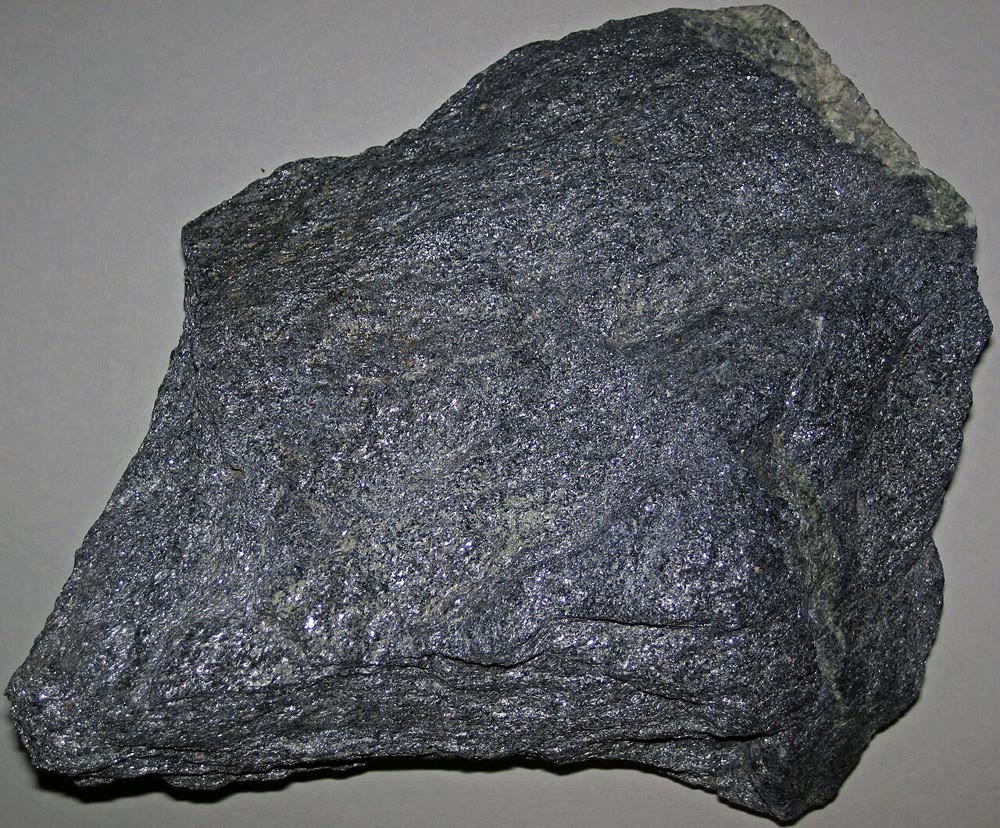
\includegraphics[width=0.27\linewidth]{images/book4/b2-10-blueschist.jpg}\hspace{0.02\linewidth}%
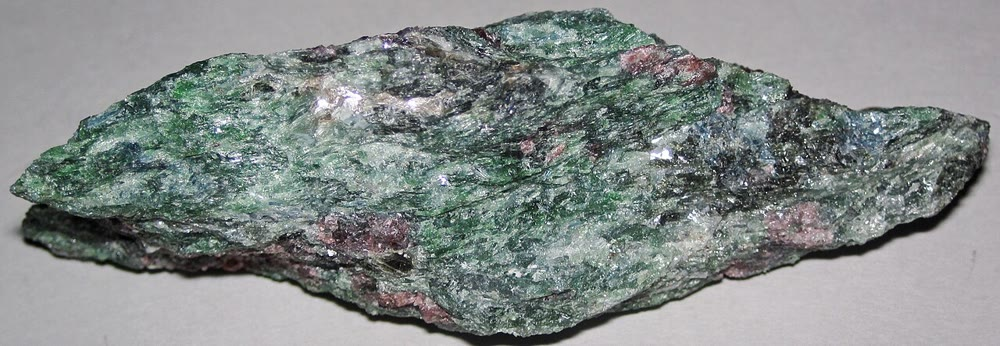
\includegraphics[width=0.69\linewidth]{images/book4/b2-10-eclogite.jpg}
\par\smallskip{\small Dua basal yang termetamorfosis. Kiri: sekis biru lawsonit dari
Kompleks Franciscan di California, biru oleh glaukofan. Kanan: eklogit dari Norwegia
bagian barat, omfasit hijau dan garnet merah dengan sedikit kuarsa, kianit, dan rutil. Foto:
James St.~John, CC BY 2.0.}
\end{omfigure}

Batuan yang terkubur dan terpanaskan bersama melewati fasies-fasies dalam urutan yang teratur, yang
mencerminkan rasio tekanan terhadap suhu di sepanjang lintasannya: tinggi di zona
subduksi, tempat sekis biru terbentuk; sedang di sabuk tumbukan; rendah di dekat intrusi.
\Cref{ch:b2:pt-paths} menamai seri-seri ini dan membaca lintasan semacam itu dari mineral.
% ledger: scmr:facies

\section{Protolit itu penting}\label{sec:b2:metamorphic-facies:protoliths}

Fasies didefinisikan berdasarkan basal, tetapi setiap \omterm{def:b2:metamorphic-facies:metamorphism}{protolit} merekam kondisi yang sama dalam
mineral-mineralnya sendiri.

\begin{definition}[Metapelit; metabasit]\label{def:b2:metamorphic-facies:protoliths}
Yang disebut \emph{metapelit}\index{metapelit} adalah batu lumpur (pelit) yang termetamorfosis, kaya akan
aluminium dan kalium, yang \omterm{def:b2:metamorphic-facies:assemblage}{himpunan mineralnya} memuat mika, klorit, garnet, staurolit, dan
aluminosilikat. Yang disebut \emph{metabasit}\index{metabasit} adalah basal,
gabro, atau batuan mafik lain yang termetamorfosis, kaya akan kalsium, magnesium, dan besi, yang \omterm{def:b2:metamorphic-facies:assemblage}{himpunan mineralnya} menentukan
fasies.
\end{definition}

Dalam \omterm{def:b2:metamorphic-facies:protoliths}{metapelit}, mineral indeks dari volume sekolah menengah atas muncul berurutan ketika
derajat \omterm{def:b2:metamorphic-facies:metamorphism}{metamorfisme} naik (klorit, biotit, garnet, staurolit, kianit, silimanit), reaksi
muskovit + kuarsa dalam bab ini menghasilkan silimanit dan feldspar-K pada suhu
yang lebih tinggi lagi, dan aluminosilikat yang hadir menunjukkan di sisi mana titik
tripel batuan itu lewat. Batu gamping atau batu dolomit yang termetamorfosis menjadi marmer, dari kalsit atau
dolomit; karbonat tidak murni, dengan silika dan lempung, menjadi batuan kalk-silikat yang
reaksi dekarbonasinya melepaskan karbon dioksida; batu pasir kuarsa menjadi kuarsit,
yang hampir tidak memperlihatkan apa pun selain ukuran butirnya. \omterm{def:b2:metamorphic-facies:protoliths}{Metapelit} zona klorit dan
metabasal di sebelahnya, pada tekanan dan suhu yang sama, sama sekali tidak mirip;
yang kedua adalah batu hijau dari aktinolit, klorit, epidot, dan albit: satu kondisi,
dua \omterm{def:b2:metamorphic-facies:assemblage}{himpunan mineral}.
% ledger: iugs:barrow, day73:ms-qz, scmr:facies-assemblages

\section{Latihan}

\begin{exercise}[$\star$]\label{exo:b2:metamorphic-facies:1}
Sebutkan jenis \omterm{def:b2:metamorphic-facies:metamorphism}{metamorfismenya}: (a) batu gamping yang terekristalisasi menjadi marmer dalam jarak
\qty{500}{m} dari sebuah granit; (b) batuan berbutir halus dan berpita di sepanjang sesar mendatar
besar, yang butirannya hancur dan terekristalisasi; (c) basal kerak samudra yang
kacanya telah berubah menjadi klorit dan zeolit di dekat punggungan, dengan mineral yang hanya sebagian
tergantikan; (d) batu pasir vulkanik di dasar tumpukan setebal \qty{10}{km}, yang
terekristalisasi tanpa skistositas.
\end{exercise}
% ledger: scmr:types

\begin{exercise}[$\star$]\label{exo:b2:metamorphic-facies:2}
Dari tabel aluminosilikat, hitunglah $\Delta_r S$, $\Delta_r V$, dan
\omterm{def:b2:metamorphic-facies:clapeyron}{kemiringan Clapeyron} kianit $\to$ silimanit, dalam \unit{bar/K} dan dalam \unit{MPa/K}. Berapa
besar perubahan tekanan kesetimbangan dalam rentang \qty{100}{\celsius}?
\end{exercise}
% ledger: rh95:al2sio5

\begin{exercise}[$\star$]\label{exo:b2:metamorphic-facies:3}
Ke fasies mana setiap metabasal termasuk? (a) aktinolit, albit, klorit, dan
epidot; (b) glaukofan dan lawsonit; (c) hornblende dan plagioklas dengan
\qty{30}{\percent} anortit; (d) omfasit dan garnet, tanpa plagioklas.
\end{exercise}
% ledger: scmr:facies-assemblages

\begin{exercise}[$\star$]\label{exo:b2:metamorphic-facies:4}
(a) Dari massa molar \qty{162.046}{g.mol^{-1}} dan volume molar 44.15, 51.52, dan
\qty{49.86}{cm^3.mol^{-1}}, hitunglah massa jenis kianit, andalusit, dan silimanit.
(b) Mineral mana yang diuntungkan oleh tekanan, dan mengapa? (c) Basis data mineral memberikan 3.61, 3.15, dan
\qty{3.24}{g.cm^{-3}}: mengapa kristal alami dapat berbeda dari fase murninya?
\end{exercise}
% ledger: rh95:al2sio5, webmineral:polymorphs

\begin{exercise}[$\star\star$]\label{exo:b2:metamorphic-facies:5}
Untuk kianit $\to$ andalusit, $\Delta_r H = \qty{3.9}{kJ}$, $\Delta_r S =
\qty{8.59}{J.K^{-1}}$, $\Delta_r V = \qty{0.737}{J.bar^{-1}}$. (a) Polimorf mana yang
stabil pada \qty{25}{\celsius} dan \qty{1}{bar}? (b) Pada suhu berapa keduanya
berdampingan pada \qty{1}{bar}? (c) Hitunglah tekanan kesetimbangan pada \qty{400}{\celsius} dan
bandingkan dengan nilai eksperimental \qty{2.54}{kbar}. (d) Mengapa andalusit tetap
dijumpai dalam batuan yang telah mendingin sampai ke permukaan?
\end{exercise}
% ledger: rh95:al2sio5, hm93:table11

\begin{exercise}[$\star\star$]\label{exo:b2:metamorphic-facies:6}
Ujilah langkah (2) metode itu. Pada \qty{1000}{K} tabel memberikan $S_T$ = 285.02 untuk kianit
dan 296.44 untuk silimanit, serta $(H_T - H_{298})/T$ = 122.29 dan 121.39
(\unit{J.mol^{-1}.K^{-1}}). (a) Hitunglah $\Delta_r H$, $\Delta_r S$, dan $\Delta_r G$
kianit $\to$ silimanit pada \qty{1000}{K} dan \qty{1}{bar}. (b) Bandingkan dengan nilai
konstan dalam tabel. (c) Polimorf mana yang stabil di sana, dan seberapa besar galat
metode sederhana itu?
\end{exercise}
% ledger: rh95:al2sio5-ht, rh95:al2sio5

\begin{exercise}[$\star\star$]\label{exo:b2:metamorphic-facies:7}
Kalsit dan aragonit (\ce{CaCO3}) pada \qty{298.15}{K} memiliki $\Delta_f G$ = $-1128.5$ dan
$-1127.4$ \unit{kJ.mol^{-1}}, $S$ = 91.7 dan 88.0 \unit{J.mol^{-1}.K^{-1}}, $V$ = 36.93
dan \qty{34.15}{cm^3.mol^{-1}}, serta entalpi pembentukan yang sama. (a) Tentukan
tekanan kesetimbangan pada \qty{25}{\celsius}. (b) Hitunglah \omterm{def:b2:metamorphic-facies:clapeyron}{kemiringan Clapeyron}. (c) Tentukan
tekanan kesetimbangan pada \qty{300}{\celsius}. (d) Banyak cangkang terbuat dari aragonit dan
hidup pada \qty{1}{bar}: apa artinya hal itu?
\end{exercise}
% ledger: rh95:cc-ar

\begin{exercise}[$\star\star$]\label{exo:b2:metamorphic-facies:8}
Untuk albit $\to$ jadeit + kuarsa, tabel memberikan $\Delta_r H = \qty{-5.0}{kJ}$,
$\Delta_r S = \qty{-32.4}{J.K^{-1}}$, $\Delta_r V = \qty{-1.698}{J.bar^{-1}}$. (a)
Hitunglah \omterm{def:b2:metamorphic-facies:clapeyron}{kemiringan Clapeyron}. (b) Hitunglah tekanan kesetimbangan pada \qty{500}{\celsius}.
(c) Entalpi pembentukan albit, jadeit, dan kuarsa memiliki ketidakpastian 2.6, 3.6,
dan \qty{1.0}{kJ.mol^{-1}}; bila digabungkan sebagai galat yang saling independen, seberapa besar ketidakpastian
tekanan itu? (d) Mengapa fasies eklogit tidak mengandung plagioklas?
\end{exercise}
% ledger: rh95:ab-jd-qz, scmr:facies-assemblages

\begin{exercise}[$\star\star$]\label{exo:b2:metamorphic-facies:9}
Muskovit + kuarsa terurai pada 603, 637, dan \qty{662}{\celsius} pada 1, 2, dan
\qty{3}{kbar}. (a) Hitunglah kemiringan garis di antara setiap pasangan titik. (b) Jika
entropi reaksi hampir tidak berubah dalam rentang ini, dengan faktor berapa $\Delta_r V$
menyusut dari selang pertama ke selang kedua? (c) Fase mana yang bertanggung jawab?
\end{exercise}
% ledger: day73:ms-qz

\begin{exercise}[$\star\star\star$]\label{exo:b2:metamorphic-facies:10}
Dengan sifat-sifat konstan menurut metode itu: (a) hitunglah tekanan ketiga
reaksi pada \qty{600}{\celsius}; (b) tunjukkan bahwa pada \qty{600}{\celsius} dan tekanan
kianit $=$ andalusit, silimanit adalah polimorf yang paling stabil, sehingga titik
tersebut pada garis itu metastabil; (c) polimorf mana yang stabil pada \qty{600}{\celsius} dan
\qty{4}{kbar}, dan pada \qty{600}{\celsius} dan \qty{7}{kbar}?
\end{exercise}
% ledger: rh95:al2sio5

\begin{exercise}[$\star\star\star$]\label{exo:b2:metamorphic-facies:11}
Sebuah sekis mengandung kianit, andalusit, dan silimanit bersama-sama, ketiganya tumbuh dalam
kesetimbangan. (a) Dengan titik tripel eksperimental, $504 \pm \qty{20}{\celsius}$ dan
$3.75 \pm \qty{0.25}{kbar}$, dan kerak bermassa jenis \qty{2700}{kg.m^{-3}} ($g =
\qty{9.81}{m.s^{-2}}$), pada kedalaman berapa sekis itu tumbuh? (b) Dengan suhu \qty{10}{\celsius} di
permukaan, gradien termal rata-rata berapa yang tersirat? (c) Mengapa batuan semacam itu jarang?
\end{exercise}
% ledger: hm93:triple

\begin{exercise}[$\star\star\star$]\label{exo:b2:metamorphic-facies:12}
Dua batuan terkubur sampai kedalaman $z$, mulai dari \qty{10}{\celsius} di permukaan: batuan X menyusuri
\qty{10}{\celsius.km^{-1}} sampai \qty{30}{km} di bawah batuan bermassa jenis rata-rata
\qty{3000}{kg.m^{-3}}, batuan Y menyusuri \qty{30}{\celsius.km^{-1}} sampai \qty{20}{km} di bawah batuan
bermassa jenis rata-rata \qty{2800}{kg.m^{-3}}. (a) Hitunglah $T$ dan $P$ pada akhir setiap lintasan.
(b) Dengan garis-garis bersifat konstan (kalsit $=$ aragonit: $P = 13.31\,T$ bar dengan $T$
dalam kelvin; albit $=$ jadeit + kuarsa dari \cref{exo:b2:metamorphic-facies:8}; aluminosilikat dari
tabel), manakah di antara aragonit atau kalsit, jadeit + kuarsa atau albit, dan
aluminosilikat mana yang dikandung setiap batuan? (c) Lintasan mana yang lebih dingin dan bertekanan tinggi, dan di fasies mana masing-masing berakhir?
\end{exercise}
% ledger: rh95:cc-ar, rh95:ab-jd-qz, rh95:al2sio5

\section{Soal: Membangun titik tripel}

\begin{problem}[{Soal akhir pekan --- diagram aluminosilikat dari tabel, dan seberapa
jauh diagram itu dapat dipercaya}]
\label{pb:b2:metamorphic-facies:1}
Gunakan tabel aluminosilikat (\qty{298.15}{K}, \qty{1}{bar}) dan metode
bab ini, dengan $\Delta_r H$, $\Delta_r S$, dan $\Delta_r V$ yang konstan; tuliskan $T$ dalam
kelvin, $P$ dalam bar, dan abaikan angka 1 dalam $P - 1$.

\noindent\textbf{Bagian I --- Reaksi-reaksinya.}
\begin{enumerate}
\item Hitunglah $\Delta_r H$, $\Delta_r S$, dan $\Delta_r V$ untuk kianit $\to$ andalusit.
\item Lakukan hal yang sama untuk kianit $\to$ silimanit.
\item Lakukan hal yang sama untuk andalusit $\to$ silimanit, dan periksalah bahwa setiap sifat adalah
selisih dari dua yang pertama.
\item Polimorf mana yang entropinya paling besar, mana yang volumenya paling kecil? Di sisi mana
dari setiap garis masing-masing polimorf itu akan terletak?
\item Hitunglah ketiga \omterm{def:b2:metamorphic-facies:clapeyron}{kemiringan Clapeyron}.
\item Mengapa kemiringan andalusit $\to$ silimanit negatif?
\end{enumerate}

\noindent\textbf{Bagian II --- Letak garis-garisnya.}
\begin{enumerate}[resume]
\item Hitunglah $\Delta_r G$ dua reaksi pertama pada \qty{298.15}{K}. Polimorf
mana yang stabil di permukaan?
\item Pada suhu berapa (dalam \unit{\celsius}) setiap reaksi mencapai kesetimbangan pada
\qty{1}{bar}?
\item Dari ketiga suhu pada pertanyaan~8, mana yang merupakan kesetimbangan stabil dan mana yang
metastabil? (Gunakan urutan ketiganya pada \qty{1}{bar}.)
\item Hitunglah tekanan kianit $=$ andalusit pada \qty{400}{\celsius}; percobaan
memberikan \qty{2.54}{kbar}.
\item Hitunglah tekanan kianit $=$ silimanit pada \qty{700}{\celsius}; percobaan
memberikan \qty{7.86}{kbar}.
\item Sketsalah ketiga garis itu antara 200 dan \qty{900}{\celsius}.
\end{enumerate}

\noindent\textbf{Bagian III --- Titik tripel.}
\begin{enumerate}[resume]
\item Tuliskan dua garis pertama sebagai $P = a_i T - b_i$; berikan $a_1$, $b_1$, $a_2$, $b_2$.
\item Selesaikan untuk memperoleh suhu titik potongnya.
\item Hitunglah tekanannya.
\item Periksalah bahwa garis andalusit $=$ silimanit melaluinya.
\item Bandingkan dengan nilai eksperimental $504 \pm \qty{20}{\celsius}$ dan $3.75 \pm
\qty{0.25}{kbar}$.
\item Dengan ketergantungan pada suhu menurut tabel, titik tripel bergeser ke
\qty{536}{\celsius} dan \qty{4.20}{kbar}. Apakah penyempurnaan itu membawanya lebih dekat ke
hasil percobaan? Apa yang diisyaratkan hal itu tentang sumber galat utama?
\end{enumerate}

\noindent\textbf{Bagian IV --- Seberapa jauh dapat dipercaya.}
\begin{enumerate}[resume]
\item Naikkan entalpi pembentukan andalusit sebesar \qty{1}{kJ}. Seberapa jauh
garis kianit $=$ andalusit bergeser dalam tekanan, pada suhu tetap?
\item Seberapa jauh titik tripel bergeser dalam suhu?
\item Lakukan hal yang sama untuk kenaikan \qty{1}{kJ} pada entalpi silimanit.
\item Setiap entalpi memiliki ketidakpastian \qty{2.0}{kJ}. Rentang suhu titik tripel
berapa yang diizinkan oleh data kalorimetri saja?
\item Lalu bagaimana tabel termodinamika dapat mereproduksi diagram eksperimental dalam selisih
\qty{30}{\celsius}?
\item Nyatakan suhu titik tripel yang dihitung pada Bagian III, dibulatkan sampai
derajat terdekat: angka kunci soal ini.
\end{enumerate}
\end{problem}
% ledger: rh95:al2sio5, rh95:al2sio5-ht, hm93:triple, hm93:table11, hm93:adjusted
